\documentclass[english, aspectratio=169]{beamer}
% english is for the language used in standard texts (figures, tables etc)
% aspectratio of 16:9 or set it for more old school to 4:3 (without the ':')

% ---------------------------------------------------------------------------- %
% Load base preamble
% ---------------------------------------------------------------------------- %
\usepackage{import}
\subimport{./preamble/}{beamer.tex}

\metroset{sectionpage=none}

% ---------------------------------------------------------------------------- %
% Local settings
% ---------------------------------------------------------------------------- %
% https://tex.stackexchange.com/a/20613
\newcommand\hcancel[2][black]{\setbox0=\hbox{$#2$}%
  \rlap{\raisebox{.35\ht0}{\textcolor{#1}{\rule{\wd0}{1pt}}}}#2}

\newcommand{\B}[0]{\ensuremath{\mathbb{B}}}

\newcommand{\sort}[0]{\text{sort}}

\newcommand{\triple}[3]{\ensuremath{(#1, #2, #3)}}
\renewcommand{\arc}[3]{\ensuremath{#1 \xrightarrow{_{#2}} #3}}

\tikzstyle{plot_adiar}=[color=black, mark=o, mark size=1pt, line width=0.7pt]
\tikzstyle{plot_buddy}=[color=red, mark=o, mark size=1pt, line width=0.7pt]
\tikzstyle{plot_cudd}=[color=blue, mark=diamond, mark size=1pt, line width=0.7pt]
\tikzstyle{plot_sylvan}=[color=purple, mark=square, mark size=1pt, line width=0.7pt]

% Horizontal legends: https://tex.stackexchange.com/a/101578
% argument #1: any options
\makeatletter
\newenvironment{customlegend}[1][]{%
    \begingroup
    % inits/clears the lists (which might be populated from previous
    % axes):
    \pgfplots@init@cleared@structures
    \pgfplotsset{#1}%
}{%
    % draws the legend:
    \pgfplots@createlegend
    \endgroup
}%

% makes \addlegendimage available (typically only available within an
% axis environment):
\def\addlegendimage{\pgfplots@addlegendimage}
\makeatother

% ------------------------------------------------------------------------------
% TITLEPAGE
% ------------------------------------------------------------------------------
\title{
  I/O-efficient Manipulation of Binary Decision Diagrams
  \\
  {\normalsize Steffan Christ S{\o}lvsten}
}

\author{
  S. C. S{\o}lvsten, J. van de Pol, A. B. Jakobsen, and M. W. B. Thomasen.
  \\
  \emph{Adiar: Binary Decision Diagrams in External Memory}. 2022
}

\institute{
\includegraphics[width=0.2\linewidth]{external/aulogo_uk_var2_black.eps}}

\date{}

\begin{document}

\titleframe

\blankframe

\begin{frame}[plain,noframenumbering]{}
  \frametitle{Contents}
  \tableofcontents
\end{frame}

\section{What are Binary Decision Diagrams?}

\begin{frame}[plain,noframenumbering]{}
  \frametitle{Contents}
  \tableofcontents[currentsection]
\end{frame}

\begin{frame}
  %Representation of functions $\B^n \rightarrow \B$ by Bryant '86.

  \begin{figure}
    \centering

    \begin{subfigure}{0.49\linewidth}
      \centering

      \begin{tikzpicture}[scale=0.8, every node/.style={transform shape}]
          % nodes
  \node[shape = circle, draw = black]
  (0) {$x_0$};

  \node[shape = circle, draw = black, below right= .4cm and .5cm of 0]
  (1) {$x_1$};

  \node[shape = circle, draw = black, below left=.4cm and .5cm of 1]
  (2) {$x_2$};

  \node[shape = circle, draw = black, below left=.4cm and .5cm of 2]
  (31) {$x_3$};
  \node[shape = circle, draw = black, below right=.4cm and .5cm of 2]
  (32) {$x_3$};

  % leafs
  \node[shape = rectangle, draw = black, below=.4cm of 31]
  (sink_T) {$\top$};

  \node[shape = rectangle, draw = black, below=.4cm of 32]
  (sink_F) {$\bot$};

  % arcs
  \draw[->, dashed]
    (0)  edge (2)
    (1)  edge (2)
    (2)  edge (31)
    (31) edge (sink_T)
    (32) edge (sink_F)
  ;

  \draw[->]
    (0)  edge (1)
    (1)  edge (32)
    (2)  edge (32)
    (31) edge (sink_F)
    (32) edge (sink_T)
  ;
      \end{tikzpicture}

      \caption{$(x_0 \wedge x_1 \wedge x_3) \vee (x_2 \oplus x_3)$}
    \end{subfigure}
    \begin{subfigure}{0.49\linewidth}
      \centering

      \begin{tikzpicture}[scale=0.8, every node/.style={transform shape}]
          % nodes
  \node[shape = circle, draw = black]
  (0) {$x_0$};

  \node[shape = circle, draw = black, below left=1.4cm and .5cm of 0]
  (21) {$x_2$};

  \node[shape = circle, draw = black, below right=1.4cm and .5cm of 0]
  (22) {$x_2$};

  \node[shape = circle, draw = black, below right=0.4cm and .5cm of 21]
  (3) {$x_3$};

  % leafs
  \node[shape = rectangle, draw = black, below right=.4cm and .5cm of 3]
  (sink_F) {$\bot$};

  \node[shape = rectangle, draw = black, below left=.4cm and .5cm of 3]
  (sink_T) {$\top$};

  % arcs
  \draw[->, dashed]
    (0)  edge (21)
    (21) edge (sink_T)
    (22) edge (3)
    (3)  edge (sink_T)
  ;

  \draw[->]
    (0)  edge (22)
    (21) edge (3)
    (22) edge (sink_F)
    (3)  edge (sink_F)
  ;
      \end{tikzpicture}

      \caption{$\neg(x_0\ ?\ x_2 \wedge x_3 : x_2 \wedge x_3)$}
    \end{subfigure}

    \caption{Examples of (Reduced Ordered) Binary Decision Diagrams.}
  \end{figure}
\end{frame}

\begin{frame}
  \begin{theorem}[Bryant '86]
    For a fixed variable order, if one exhaustively applies the two rules below,
    then one obtains the Reduced OBDD, which is a unique canonical form of the
    function.
  \end{theorem}

  \begin{figure}
    \centering

    \begin{subfigure}[b]{0.40\linewidth}
      \centering

      \begin{tikzpicture}[scale=0.9, every node/.style={transform shape}]
        \node[shape = circle, black, draw = black] (i) {$x_i$};
\node[shape = circle, draw = black, below=of i] (child) {};
\node[shape = circle, draw = black, above=of i] (parent) {};

% implication
\node[shape = circle, black,right=0.5cm of i] {$\implies$};

% after
\node[shape = circle, draw = black, right=2.5cm of child] (childafter) {};
\node[shape = circle, draw = black, right=2.5cm of parent] (parentafter) {};

\draw[->, dashed] (i) edge[bend right] (child);
\draw[->]
(i) edge[bend left] (child)
(parent) edge (i)
(parentafter) edge (childafter)
;

      \end{tikzpicture}

      \vspace{10pt}
      {\small {\bf (1)} Remove redundant nodes}
    \end{subfigure}
    \begin{subfigure}[b]{0.59\linewidth}
      \centering

      \begin{tikzpicture}[scale=0.9, every node/.style={transform shape}]
        \node[shape = circle, black, draw = black] (i1) {$x_i$};
\node[shape = circle, black, draw = black, right=of i1] (i2) {$x_i$};

\node[shape = circle, draw = black, below=of i1] (child1) {};
\node[shape = circle, draw = black, below=of i2] (child2) {};

\node[shape = circle, draw = black, above=of i1] (parent1) {};
\node[shape = circle, draw = black, above=of i2] (parent2) {};

% implication
\node[shape = circle, black,right=0.5cm of i2] {$\implies$};

% after
\node[shape = circle, draw = black, right=4cm of child1] (c1a) {};
\node[shape = circle, draw = black, right=4cm of child2] (c2a) {};

\node[shape = circle, black, draw = black, right=2.7cm of i2] (ia) {$x_i$};

\node[shape = circle, draw = black, right=4cm of parent1] (p1a) {};
\node[shape = circle, draw = black, right=4cm of parent2] (p2a) {};


\draw[->, dashed]
(i1) edge (child1)
(i2) edge (child1)
(ia) edge (c1a)
;
\draw[->]
(i1) edge (child2)
(i2) edge (child2)
(parent1) edge (i1)
(parent2) edge (i2)
(p1a) edge (ia)
(p2a) edge (ia)
(ia) edge (c2a)
;

      \end{tikzpicture}

      \vspace{10pt}
      {\small {\bf (2)} Merge duplicate nodes}
    \end{subfigure}

  \end{figure}

\end{frame}

\begin{frame}[t]
  \frametitle{\texttt{bdd\_apply(f,g,$\odot$)}}

  \textbf{Base Case ($f,g \in \B$):}
  \begin{figure}
    \centering

    \begin{tikzpicture}
      % 'f'
      \node at (0,0) (f) {$\alpha$};

      \node at (0,1) (fp) {};
      \draw[->] (fp) edge (f);

      % 'odot'
      \node at (1,0) {$\odot$};

      % 'g'
      \node at (2,0) (g) {$\beta$};

      \node at (2,1) (gp) {};
      \draw[->] (gp) edge (g);

      \node at (3.4,0) {$\mapsto$};

      % 'f \odot g'
      \node at (5.25,0) (fg) {$\alpha \odot \beta$};

      \node at (5.25,1) (fgp) {};
      \draw[->] (fgp) edge (fg);
    \end{tikzpicture}
  \end{figure}

  \textbf{Inductive Case:}
  \begin{figure}
    \centering

    \begin{tikzpicture}
      % 'f'
      \node[shape = circle, draw = black] at (0,0) (f) {$x_i$};

      \node at (-0.5,-1) (f0) {$\alpha$};
      \node at (0.5,-1) (f1) {$\beta$};

      \draw[->, dashed] (f) edge (f0);
      \draw[->]         (f) edge (f1);

      \node at (0,1) (fp) {};
      \draw[->] (fp) edge (f);

      % 'odot'
      \node at (1,0) {$\odot$};

      % 'g'
      \only<1>{
        \node[shape = circle, draw = black] at (2,0) (g) {$x_i$};

        \node at (1.5,-1) (g0) {$\gamma$};
        \node at (2.5,-1) (g1) {$\delta$};

        \draw[->, dashed] (g) edge (g0);
        \draw[->]         (g) edge (g1);
      }
      \only<2->{
        \node at (2,-1) (g) {$\mu$};
      }

      \node at (2,1) (gp) {};
      \draw[->] (gp) edge (g);

      \node at (3.4,0) {$\mapsto$};

      % 'f \odot g'
      \node[shape = circle, draw = black] at (5.25,0) (fg) {$x_i$};

      \node at (4.5,-1) (fg0) {$\alpha \odot \only<1>{\gamma}\only<2->{\mu}$};
      \node at (6,-1) (fg1) {$\beta \odot \only<1>{\delta}\only<2->{\mu}$};

      \draw[->, dashed] (fg) edge (fg0);
      \draw[->]         (fg) edge (fg1);

      \node at (5.25,1) (fgp) {};
      \draw[->] (fgp) edge (fg);
    \end{tikzpicture}
  \end{figure}
\end{frame}

\begin{frame}
  \frametitle{\texttt{bdd\_apply(f,g,$\odot$)}}

  Let $N_f$, $N_g$ be the size of the BDDs for $f$ and $g$.

  Let $T$ be the $O(N_f \cdot N_g)$ size of the BDD for $f \odot g$.

  \begin{theorem}
    \lstinline{bdd_apply(f,g,}$\odot$\lstinline{)} runs in $O(N_f + N_g + T)$
    time
  \end{theorem}
  \begin{itemize}
  \item Memoisation (\emph{Computation Cache}) ensures each $(t_f,t_g)$ is
    only computed once.

  \item Reduction Rules can be maintained with a
    \texttt{make\_node($i$,$t$,$e$)} in $O(1)$ time.
    \begin{enumerate}
    \item Redundancy is resolved with an if-statement.
    \item Duplication is avoided with a hash table (\emph{Unique Node Table}).
    \end{enumerate}
  \end{itemize}

  \begin{corollary}
    \lstinline{bdd_apply(f,g,}$\odot$\lstinline{)} runs in $O(1)$ time per BDD node.
  \end{corollary}
\end{frame}

\blankframe

\begin{frame}%[plain,noframenumbering]{} % \blankframe until reveal
  \begin{center}
    {\fontsize{42}{50}\selectfont \textbf{Adiar}}

    \textcolor{gray}{\large \em
      I/O-efficient Decision Diagrams
    }

    \vspace{-10pt}
    \rule{180pt}{0.6pt}
    \vspace{-5pt}

    \textcolor{gray}{\small
      \href{http://github.com/ssoelvsten/adiar}{github.com/ssoelvsten/adiar}
    }
  \end{center}
\end{frame}

\begin{frame}
  \begin{figure}
    \centering

    \begin{tikzpicture}
      \begin{axis}[%
        width=0.69\linewidth, height=0.42\linewidth,
        every tick label/.append style={font=\scriptsize},
        % x-axis
        xlabel={Number of BDD Nodes},
        xmajorgrids=true,
        xmin=800000 ,
        xmax=1200000000,
        xmode = log,
        % y-axis
        ymin=0.1,
        ymax=0.27,
        ylabel={$\mu$s / BDD Node},
        ytick distance={0.05},
        yminorgrids=false,
        ymajorgrids=true,
        grid style={dashed,black!20},
        ]

        \addplot [style=plot_buddy]
        table {./data/cache_buddy_time_per_node.tex};
      \end{axis}
    \end{tikzpicture}

    \caption{Running time of \emph{BuDDy} for the $N$-Queens problem.}
  \end{figure}
\end{frame}

\begin{frame}
  \begin{figure}
    \centering

    \begin{tikzpicture}
      \begin{axis}[%
        width=0.69\linewidth, height=0.42\linewidth,
        every tick label/.append style={font=\scriptsize},
        % x-axis
        xlabel={Memory (GiB)},
        xmajorgrids=true,
        xmin=3.5,
        xmax=10.5,
        xtick={4, ..., 10},
        % y-axis
        ylabel={time (seconds)},
        yminorgrids=false,
        ymajorgrids=true,
        grid style={dashed,black!20},
        ]

        \draw [white, pattern=north west lines, pattern color=black!30!white]
        (axis cs: 8, 0) rectangle (axis cs: 10, 3000);

        \addplot[thick, samples=1, smooth, black, name path=barrier]
        coordinates {(8,0)(8,3000)};

        \node[black] at (axis cs: 7.6, 2800){\tiny{RAM}};
        \node[black] at (axis cs: 8.4, 2800){\tiny{Swap}};

        \addplot [style=plot_buddy]
        table {./data/cache_buddy_swap.tex};
      \end{axis}
    \end{tikzpicture}

    \caption{Running time of \emph{BuDDy} for \emph{3D Tic-Tac-Toe} with $N=21$.}
  \end{figure}
\end{frame}

\section{Why do they break?}

\begin{frame}[plain,noframenumbering]{}
  \frametitle{Contents}
  \tableofcontents[currentsection]
\end{frame}

\begin{frame}
  % Numbers from:
% - Intel® 64 and IA-32 Architectures Optimization Reference Manual
%   + Cache: Table 2-7/2-14
%   + RAM:   3.6.10 Locality Enhancement
% - www.lighterra.com/papers/modernmicroprocessors/
%   + SSD: Extrapolation from the 2.000.000 to fit Intel's Manual.
% - imada.sdu.dk/u/rolf/Edu/DM79/E04/Slides/IOModel.pdf
%   + HDD: Extrapolation from the 2.000.000 to fit Intel's Manual.

\begin{center}
  \begin{tikzpicture}
    % ALU
    \node[draw, trapezium, shape border rotate=180, text width=0.8cm, align=center] at (0,0) (cpu) {CPU};

    % Cache
    \draw[draw=gray, rounded corners=3pt, densely dotted, line width = 0.6pt]
    (-1.3,2.3) rectangle ++(2.6,-1.6);

    \node[ draw, rectangle, text width=0.3cm, align=center] at (0,1)    (l1) {\tiny L1};
    \node[ draw, rectangle, text width=0.8cm, align=center] at (0,1.45) (l2) {\tiny L2};
    \node[ draw, rectangle, text width=2cm, align=center]   at (0,1.95) (l3) {\footnotesize L3};

    \path[->]
    (cpu) edge[bend left=25] (l1)
    (l1) edge[bend left=25] (cpu) ;
    \onslide<2->{\node at (2.8,0.5) {$\sim$ 4 -- 50 CPU Cycles};}

    % Main memory
    \node[draw, rectangle, text width=4cm, align=center] at (0,3.5) (ram) {RAM};

    \path[->]
      (l3) edge[bend left=40] (ram)
      (ram) edge[bend left=40] (l3)
    ;
    \onslide<2->{
      \node at (2.6,2.7) {$\sim$ 200 CPU Cycles};
    }

    % Disk
    \only<-2> { \node[ draw, cylinder, minimum width=8cm, aspect=0.3,
      align=center, shape border rotate=90 ] at (0,5.5) (disk) {SSD};
    }
    \onslide<3> { \node[ draw, cylinder, minimum width=12cm, aspect=0.26,
      align=center, shape border rotate=90 ] at (0,5.5) (disk) {HDD};
    }

    \path[->]
      (disk) edge[bend left=40] (ram)
      (ram) edge[bend left=40] (disk)
    ;
    \only<2>{
      \node at (3,4.5) {$\sim$ 200.000+ CPU Cycles};
    }
    \onslide<3->{
      \node at (3.25,4.5) {$\sim$ 20.000.000+ CPU Cycles};
    }
  \end{tikzpicture}
\end{center}
\end{frame}

\begin{frame}
  \begin{figure}
    \centering

    \begin{tikzpicture}
  % ALU
  \node[
  draw,
  trapezium,
  shape border rotate=180,
  text width=1cm,
  align=center,
  ] at (0.03,0) (cpu) {CPU};

  % Main memory
  \begin{scope}
    \clip(-1.13,1) rectangle (1.19,1.4);
    \filldraw[
    color=black!60!white,
    fill=black!5!white,
    pattern=vertical lines,
    pattern color=black!30!white
    ] (-9,1.25) rectangle ++(18,0.5)
    ;
  \end{scope}

  \node[
  draw,
  rectangle,
  text width=2.08cm,
  align=center,
  ] at (0.03,1.5) (m) {$M$};

  % Disk
  \begin{scope}
    \clip(-6,2.5) rectangle (6,2.9);
    \filldraw[
    color=black!60!white,
    fill=black!5!white,
    pattern=vertical lines,
    pattern color=black!30!white
    ] (-9,2.75) rectangle ++(18,0.5)
    ;
  \end{scope}

  \node[
  draw,
  rectangle,
  text width=5.04cm,
  align=center,
  ] at (0.03,3) (n) {$N$};

  \path[->]
  (cpu) edge[bend left=40] (m)
  (m) edge[bend left=40] (cpu)

  (n) edge[bend left=40] (m)
  (m) edge[bend left=40] (n)
  ;

  \node at (0.02,2.24) {\textcolor{gray}{$B$}};
\end{tikzpicture}


    \caption{The I/O model by Aggarwal and Vitter '87}
  \end{figure}
\end{frame}

\begin{frame}
  For any realistic values of $N$, $M$, and $B$ we have that

  \begin{equation*}
      N/B \quad < \quad \sort(N) \triangleq N/B \cdot \log_{M/B} N/B \quad \ll \quad N
    \enspace ,
  \end{equation*}

  \begin{theorem}[Aggarwal and Vitter '87]
    $N$ elements can be sorted in $\Theta(\sort(N))$ I/Os.
  \end{theorem}
  \begin{theorem}[Arge '95]
    A Priority Queue can do $N$ insertions and extractions in $\Theta(\sort(N))$
    I/Os.
  \end{theorem}
\end{frame}

\begin{frame}[fragile]
  \frametitle{CountPaths : \emph{Example}}

  \begin{columns}
  \begin{column}{0.49\textwidth}
    \begin{figure}
      \centering

      \begin{subfigure}{1\linewidth}
        \centering

        \begin{tikzpicture}[scale=0.9, every node/.style={transform shape}]
          % blocks
          \draw[draw=gray, dashed] (-0.45,-0.45) rectangle ++(1.3,0.9);
          \draw[draw=gray, dashed] (-0.45,-2.35) rectangle ++(1.95,1.85);
          \draw[draw=gray, dashed] (-1.5,-3.32) rectangle ++(3,0.9);
          \draw[draw=gray, dashed] (-1.5,-4.35) rectangle ++(3,0.9);

          % nodes
            % nodes
  \node[shape = circle, draw = black]
  (0) {$x_0$};

  \node[shape = circle, draw = black, below right= .4cm and .5cm of 0]
  (1) {$x_1$};

  \node[shape = circle, draw = black, below left=.4cm and .5cm of 1]
  (2) {$x_2$};

  \node[shape = circle, draw = black, below left=.4cm and .5cm of 2]
  (31) {$x_3$};
  \node[shape = circle, draw = black, below right=.4cm and .5cm of 2]
  (32) {$x_3$};

  % leafs
  \node[shape = rectangle, draw = black, below=.4cm of 31]
  (sink_T) {$\top$};

  \node[shape = rectangle, draw = black, below=.4cm of 32]
  (sink_F) {$\bot$};

  % arcs
  \draw[->, dashed]
    (0)  edge (2)
    (1)  edge (2)
    (2)  edge (31)
    (31) edge (sink_T)
    (32) edge (sink_F)
  ;

  \draw[->]
    (0)  edge (1)
    (1)  edge (32)
    (2)  edge (32)
    (31) edge (sink_F)
    (32) edge (sink_T)
  ;

          % animations (nodes)
          \onslide<2>{
            \node[shape = circle, orange, draw = orange]
            {$x_0$};
          }

          \onslide<3>{
            \node[shape = circle, orange, draw = orange, below left=.4cm and .5cm of 1]
            {$x_2$};
          }

          \onslide<4>{
            \node[shape = circle, orange, draw = orange, below left=.4cm and .5cm of 2]
            {$x_3$};
          }

          \onslide<5>{
            \node[shape = rectangle, orange, draw = orange, below=.4cm of 31]
            {$\top$};
          }

          \onslide<6>{
            \node[shape = circle, orange, draw = orange, below left=.4cm and .5cm of 2]
            {$x_3$};
          }

          \onslide<7>{
            \node[shape = rectangle, orange, draw = orange, below=.4cm of 32]
            {$\bot$};
          }

          \onslide<8>{
            \node[shape = circle, orange, draw = orange, below left=.4cm and .5cm of 2]
            {$x_3$};
          }

          \onslide<9>{
            \node[shape = circle, orange, draw = orange, below left=.4cm and .5cm of 1]
            {$x_2$};
          }

          \onslide<10>{
            \node[shape = circle, orange, draw = orange, below right=.4cm and .5cm of 2]
            {$x_3$};
          }

          \onslide<11>{
            \node[shape = rectangle, orange, draw = orange, below=.4cm of 32]
            {$\bot$};
          }

          \onslide<12>{
            \node[shape = circle, orange, draw = orange, below right=.4cm and .5cm of 2]
            {$x_3$};
          }

          \onslide<13>{
            \node[shape = rectangle, orange, draw = orange, below=.4cm of 31]
            {$\top$};
          }

          \onslide<14>{
            \node[shape = circle, orange, draw = orange, below right=.4cm and .5cm of 2]
            {$x_3$};
          }

          \onslide<15>{
            \node[shape = circle, orange, draw = orange, below left=.4cm and .5cm of 1]
            {$x_2$};
          }

          \onslide<16>{
            \node[shape = circle, orange, draw = orange]
            {$x_0$};
          }

          \onslide<17>{
            \node[shape = circle, orange, draw = orange, below right= .4cm and .5cm of 0]
            {$x_1$};
          }

          \onslide<18>{
            \node[shape = circle, orange, draw = orange, below left=.4cm and .5cm of 1]
            {$x_2$};
          }

          \onslide<19>{
            \node[shape = circle, orange, draw = orange, below right= .4cm and .5cm of 0]
            {$x_1$};
          }

          \onslide<20>{
            \node[shape = circle, orange, draw = orange, below right=.4cm and .5cm of 2]
            {$x_3$};
          }

          \onslide<21>{
            \node[shape = circle, orange, draw = orange, below right= .4cm and .5cm of 0]
            {$x_1$};
          }

          \onslide<22>{
            \node[shape = circle, orange, draw = orange]
            {$x_0$};
          }

          % animations (I/Os)
          \onslide<2-3>{
            \draw[draw=purple] (-0.45,-0.45) rectangle ++(1.3,0.9);
          }
          \onslide<3-4>{
            \draw[draw=purple] (-0.45,-2.35) rectangle ++(1.95,1.85);
          }
          \onslide<4-15>{
            \draw[draw=purple] (-1.5,-3.32) rectangle ++(3,0.9);
          }
          \onslide<5-8>{
            \draw[draw=purple] (-1.5,-4.35) rectangle ++(3,0.9);
          }
          \onslide<9-10>{
            \draw[draw=purple] (-0.45,-2.35) rectangle ++(1.95,1.85);
          }
          \onslide<11-14>{
            \draw[draw=purple] (-1.5,-4.35) rectangle ++(3,0.9);
          }
          \onslide<15-22>{
            \draw[draw=purple] (-0.45,-2.35) rectangle ++(1.95,1.85);
          }
          \onslide<16-19>{
            \draw[draw=purple] (-0.45,-0.45) rectangle ++(1.3,0.9);
          }
          \onslide<20-21>{
            \draw[draw=purple] (-1.5,-3.32) rectangle ++(3,0.9);
          }
          \onslide<22>{
            \draw[draw=purple] (-0.45,-0.45) rectangle ++(1.3,0.9);
          }

          % animations (cache)
          \onslide<8->{
            \node[gray, right=.02cm of 31]
            {\tiny $1$};
          }

          \onslide<14->{
            \node[gray, left=.02cm of 32]
            {\tiny $1$};
          }

          \onslide<15->{
            \node[gray, right=.02cm of 2]
            {\tiny $2$};
          }

          \onslide<21->{
            \node[gray, left=.02cm of 1]
            {\tiny $3$};
          }

          \onslide<22-23>{
            \node[gray, right=.02cm of 0]
            {\tiny $5$};
          }
        \end{tikzpicture}

        \caption{$(x_0 \wedge x_1 \wedge x_3) \vee (x_2 \oplus x_3)$}
      \end{subfigure}

      %\caption{Blocks active in memory}
    \end{figure}

  \end{column}

  \begin{column}{0.49\textwidth}
    \begin{center}
      % { \small
      %   \begin{equation*}
      %     \texttt{cp}(n) =
      %     \begin{cases}
      %       1 & n = \top
      %       \\
      %       0 & n = \bot
      %       \\
      %       \texttt{cp}(n.low) + \texttt{cp}(n.high) & \text{otherwise}
      %     \end{cases}
      %   \end{equation*}
      % }

      % \vspace{20pt}

      $M = 4$, $B = 2$

      \vspace{10pt}

      \begin{tabular}{c c}
        node I/Os & cache lookups
        \\ \hline
        \only<1>{$0$}%
        \only<2>{$1$}%
        \only<3>{$2$}%
        \only<4>{$3$}%
        \only<5-8>{$4$}%
        \only<9-10>{$5$}%
        \only<11-14>{$6$}%
        \only<15>{$7$}%
        \only<16-19>{$8$}%
        \only<20-21>{$9$}%
        \only<22->{$10$}%
                  &
                    \only<1>{$0$}%
                    \only<2>{$1$}%
                    \only<3>{$2$}%
                    \only<4-9>{$3$}%
                    \only<10-16>{$4$}%
                    \only<17>{$5$}%
                    \only<18-19>{$6$}%
                    \only<20->{$7$}%
      \end{tabular}
    \end{center}

  \end{column}
\end{columns}

\end{frame}

\begin{frame}
  \begin{table}
    \centering
    \begin{tabular}{rl}
      Algorithm                 & \only<1>{Time }\only<2>{I/O-}Complexity\only<2>{\hspace{7pt}}
      \\ \hline \hline
      \lstinline{bdd_pathcount} & $O(N_f)$
      \\ \hline
      \lstinline{bdd_not}       & $O(N_f)$
      \\
      \lstinline{bdd_restrict}  & $O(N_f)$
      \\
      \lstinline{bdd_apply}     & $O(N_f \cdot N_g)$
      \\ \hline
      \lstinline{bdd_equal}     & $O(1)$
    \end{tabular}
  \end{table}
\end{frame}

\section{How can we fix it?}

\begin{frame}[plain,noframenumbering]{}
  \frametitle{Contents}
  \tableofcontents[currentsection]
\end{frame}

\subsection{CountPaths}

\begin{frame}[plain,noframenumbering]{}
  \frametitle{Contents}
  \tableofcontents[currentsection, currentsubsection]
\end{frame}

\begin{frame}
  % Let every node be uniquely identified by a tuple $(\mathit{label},
  % \mathit{id}) : \N \times \N$.

  \begin{center}
    \begin{tikzpicture}[scale=0.9, every node/.style={transform shape}]
      \node[shape = circle, black, inner sep=6pt, draw = black] (before_n) {$x_i$};
\node[shape = circle, black, draw = black, below left=1cm and 0.4cm of before_n] (before_low) {};
\node[shape = circle, black, draw = black, below right=1cm and 0.4cm of before_n] (before_high) {};

\draw[->, dashed] (before_n) edge (before_low);
\draw[->] (before_n) edge (before_high);

% implication
\node[shape = circle, black,below right=0cm and 1.2cm of before_n] (implies) {$\implies$};

% after
\node[shape = circle, black, draw = black, right=3cm of before_n] (after_n) {\tiny $(i,\mathit{id})$};
\node[shape = circle, black, draw = black, below left=0.9cm and 0.4cm of after_n] (after_low) {};
\node[shape = circle, black, draw = black, below right=0.9cm and 0.4cm of after_n] (after_high) {};

\draw[->, dashed] (after_n) edge (after_low);
\draw[->] (after_n) edge (after_high);

    \end{tikzpicture}
  \end{center}
  % Nodes are ordered based on their \emph{uid} as follows
  \vspace{20pt}
  \begin{equation*}
    (i_1, \mathit{id}_1) < (i_2, \mathit{id}_2)
    \equiv
    i_1 < i_2 \vee (i_1 = i_2 \wedge \mathit{id}_i < \mathit{id}_j)
  \end{equation*}
\end{frame}

\begin{frame}
  \begin{figure}
    \centering

    \begin{subfigure}{0.49\linewidth}
      \centering

      \begin{subfigure}[b]{0.33\linewidth}
        \centering

        \begin{tikzpicture}[scale=0.6, every node/.style={transform shape}]
            % nodes
  \node[shape = circle, draw = black]
  (0) {$x_0$};

  \node[shape = circle, draw = black, below right= .4cm and .5cm of 0]
  (1) {$x_1$};

  \node[shape = circle, draw = black, below left=.4cm and .5cm of 1]
  (2) {$x_2$};

  \node[shape = circle, draw = black, below left=.4cm and .5cm of 2]
  (31) {$x_3$};
  \node[shape = circle, draw = black, below right=.4cm and .5cm of 2]
  (32) {$x_3$};

  % leafs
  \node[shape = rectangle, draw = black, below=.4cm of 31]
  (sink_T) {$\top$};

  \node[shape = rectangle, draw = black, below=.4cm of 32]
  (sink_F) {$\bot$};

  % arcs
  \draw[->, dashed]
    (0)  edge (2)
    (1)  edge (2)
    (2)  edge (31)
    (31) edge (sink_T)
    (32) edge (sink_F)
  ;

  \draw[->]
    (0)  edge (1)
    (1)  edge (32)
    (2)  edge (32)
    (31) edge (sink_F)
    (32) edge (sink_T)
  ;
        \end{tikzpicture}
      \end{subfigure}
      \begin{subfigure}[b]{0.55\linewidth}
        \centering
        { \tiny
          \begin{tabular}{r c l}
            [ & $\triple{(0,0)}{(2,0)}{(1,0)}$ & ,
            \\ \\
              & $\triple{(1,0)}{(2,0)}{(3,1)}$ & ,
            \\ \\
              & $\triple{(2,0)}{(3,0)}{(3,1)}$ & ,
            \\ \\
              & $\triple{(3,0)}{\top}{\bot}$   & ,
            \\ \\
              & $\triple{(3,1)}{\bot}{\top}$   & ]
          \end{tabular}
          \vspace{6pt}
        }
      \end{subfigure}

      \caption{$(x_0 \wedge x_1 \wedge x_3) \vee (x_2 \oplus x_3)$}
    \end{subfigure}
    \begin{subfigure}{0.49\linewidth}
      \centering

      \begin{subfigure}[b]{0.33\linewidth}
        \centering
        \begin{tikzpicture}[scale=0.6, every node/.style={transform shape}]
            % nodes
  \node[shape = circle, draw = black]
  (0) {$x_0$};

  \node[shape = circle, draw = black, below left=1.4cm and .5cm of 0]
  (21) {$x_2$};

  \node[shape = circle, draw = black, below right=1.4cm and .5cm of 0]
  (22) {$x_2$};

  \node[shape = circle, draw = black, below right=0.4cm and .5cm of 21]
  (3) {$x_3$};

  % leafs
  \node[shape = rectangle, draw = black, below right=.4cm and .5cm of 3]
  (sink_F) {$\bot$};

  \node[shape = rectangle, draw = black, below left=.4cm and .5cm of 3]
  (sink_T) {$\top$};

  % arcs
  \draw[->, dashed]
    (0)  edge (21)
    (21) edge (sink_T)
    (22) edge (3)
    (3)  edge (sink_T)
  ;

  \draw[->]
    (0)  edge (22)
    (21) edge (3)
    (22) edge (sink_F)
    (3)  edge (sink_F)
  ;
        \end{tikzpicture}
      \end{subfigure}
      \begin{subfigure}[b]{0.55\linewidth}
        \centering
        { \tiny
          \begin{tabular}{r c l}
            [ & $((0,0), (2,0), (2,1))$ & ,
            \\ \\
              & $((2,0), \top, (3,0))$  & ,
            \\ \\
              & $((2,1), (3,0), \bot)$  & ,
            \\ \\
              & $((3,0), \top, \bot)$   & ]
          \end{tabular}
          \vspace{10pt}
        }
      \end{subfigure}

      \caption{$\neg(x_0\ ?\ x_2 \wedge x_3 : x_2 \wedge x_3)$}
    \end{subfigure}

    \caption{Node-based representation of prior shown BDDs}
  \end{figure}

\end{frame}

\begin{frame}[t]
  \frametitle{CountPaths}

  \begin{figure}
    \centering

    \begin{tikzpicture}[scale=0.9, every node/.style={transform shape}]
      % nodes
\node[shape = circle, draw = black] (n) {\small $(i,\texttt{id})$};

\node[below left  = 1 and 1 of n]  (low) {$\alpha$};
\node[below right = 1 and 1 of n] (high) {$\beta$};

% parent dummies

\node[above left  = 0.5 and 1 of n]  (p1) {$n_1$};
\node[above       = 0.5 of n] (p2) {$n_2$};
\node[above right = 0.5 and 1 of n] (p3) {$n_3$};

% arcs
\draw[->, dashed] (n) edge node[above left]{$\sum_i n_i$} (low);
\draw[->]         (n) edge node[above right]{$\sum_i n_i$} (high);

\draw[->, dotted, thick]
(p1) edge[bend left] (n)
(p2) edge (n)
(p3) edge[bend right] (n)
;

    \end{tikzpicture}
  \end{figure}

  \only<1>{
    \begin{center}
      {\Large \textbf{Idea}}

      {\large Count the number of in-going paths to each node.}
    \end{center}
  }

  \only<2->{
    \begin{center}
      {\Large \textbf{Time-Forward Processing}}

      Defer work with $Q_{\mathit{count}}$ : \texttt{PriorityQueue}$\langle (\arc{s}{}{t}, \quad
      \N) \rangle$ sorted on $t$ in ascending order.

      $(\arc{(i,\texttt{id})}{\bot}{\alpha}, \quad \sum_i n_i)$, \qquad
      $(\arc{(i,\texttt{id})}{\top}{\beta}, \quad \sum_i n_i)$
    \end{center}
  }
\end{frame}

\begin{frame}
  \frametitle{CountPaths : \emph{Example}}

  \begin{columns}
  \begin{column}{0.49\textwidth}

    \begin{figure}
      \centering

      \begin{subfigure}{1\linewidth}
        \centering

        \begin{tikzpicture}[scale=0.9, every node/.style={transform shape}]
          % nodes
          \node[shape = circle, draw = black]
          (0) {\tiny $(0,0)$};

          \node[shape = circle, draw = black, below right= .3cm and .5cm of 0]
          (1) {\tiny $(1,0)$};

          \node[shape = circle, draw = black, below left=.3cm and .5cm of 1]
          (2) {\tiny $(2,0)$};

          \node[shape = circle, draw = black, below left=.3cm and .5cm of 2]
          (31) {\tiny $(3,0)$};
          \node[shape = circle, draw = black, below right=.3cm and .5cm of 2]
          (32) {\tiny $(3,1)$};

          % leafs
          \node[shape = rectangle, draw = black, below=.4cm of 31]
          (sink_T) {$\top$};

          \node[shape = rectangle, draw = black, below=.4cm of 32]
          (sink_F) {$\bot$};

          % arcs
          \draw[->,dashed]
          (0) edge (2)
          (1) edge (2)
          (2) edge (31)
          (31) edge (sink_T)
          (32) edge (sink_F)
          ;

          \draw[->]
          (0) edge (1)
          (1) edge (32)
          (2) edge (32)
          (31) edge (sink_F)
          (32) edge (sink_T)
          ;

          % animations
          \onslide<3-5>{ % 0
            \node[shape = circle, orange, draw = orange]
            {\tiny $(0,0)$};
            \draw[->,dashed,orange] (0) edge (2);
            \draw[->,orange] (0) edge (1);
          }

          \onslide<6-9>{ % 1
            \node[shape = circle, orange, draw = orange, below right= .3cm and .5cm of 0]
            {\tiny $(1,0)$};
            \draw[->,dashed,orange] (1) edge (2);
            \draw[->,orange] (1) edge (32);
          }

          \onslide<10-14>{ % 2
            \node[shape = circle, orange, draw = orange, below left=.3cm and .5cm of 1]
            {\tiny $(2,0)$};
            \draw[->,dashed,orange] (2) edge (31);
            \draw[->,orange] (2) edge (32);
          }

          \onslide<15-18>{ % 31
            \node[shape = circle, orange, draw = orange, below left=.3cm and .5cm of 2]
            {\tiny $(3,0)$};
            \draw[->,dashed,orange] (31) edge (sink_T);
            \draw[->,orange] (31) edge (sink_F);
          }

          \onslide<19-22>{ % 32
            \node[shape = circle, orange, draw = orange, below right=.3cm and .5cm of 2]
            {\tiny $(3,1)$};
            \draw[->,dashed,orange] (32) edge (sink_F);
            \draw[->,orange] (32) edge (sink_T);
          }
        \end{tikzpicture}

        \caption{\small $(x_0 \wedge x_1 \wedge x_3) \vee (x_2 \oplus x_3)$}
      \end{subfigure}

      %\caption{In-order traversal of BDD}
    \end{figure}

  \end{column}
  \begin{column}{0.49\textwidth}
    \centering

    \onslide<5->{ \small
      \begin{tabular}{c c c}
        \onslide<5-22>{\hspace{10pt}Seek\hspace{10pt}}
        \onslide<5-22>{& \hspace{10pt}Sum\hspace{10pt}}
        \onslide<5-23>{& \hspace{10pt}Result\hspace{10pt}}
        \\
        \textcolor{orange}{%
        \only<5-8>{$(1,0)$}%
        \only<9-13>{$(2,0)$}%
        \only<14-17>{$(3,0)$}%
        \only<18-22>{$(3,1)$}%
        }
        &
        % (1,0)
          \only<5-6>{$0$}%
          \only<7-8>{$1$}%
          % (2,0)
          \only<9-10>{$0$}%
          \only<11>{$1$}%
          \only<12-13>{$2$}%
          % (3,0)
          \only<14-15>{$0$}%
          \only<16-17>{$2$}%
          % (3,1)
          \only<18-19>{$0$}%
          \only<20>{$1$}%
          \only<21-22>{$3$}%
        &
          \only<1-16>{$0$}%
          \only<17-21>{$2$}%
          \only<22-23>{$5$}%
      \end{tabular}
    }

    \vspace{20pt}

    \onslide<2->{
      {\footnotesize Priority Queue: $Q_{\mathit{count}}$:

        \begin{tabular}{rll}
          [ & \onslide<4-6>{$(\arc{(0,0)}{\top}{(1,0)}, \quad 1)$  & ,}
          \\
            & \onslide<4-10>{$(\arc{(0,0)}{\bot}{(2,0)}, \quad 1)$  & ,}
          \\
            & \onslide<8-11>{$(\arc{(1,0)}{\bot}{(2,0)}, \quad 1)$  & ,}
          \\
            & \onslide<13-15>{$(\arc{(2,0)}{\bot}{(3,0)}, \quad 2)$  & ,}
          \\
            & \onslide<8-19>{$(\arc{(1,0)}{\top}{(3,1)}, \quad 1)$   & ,}
          \\
            & \onslide<13-20>{$(\arc{(2,0)}{\top}{(3,1)}, \quad 2)$ }  & ]
        \end{tabular}
      }
    }

  \end{column}
\end{columns}

\end{frame}

\subsection{Apply}

\begin{frame}[plain,noframenumbering]{}
  \frametitle{Contents}
  \tableofcontents[currentsection, currentsubsection]
\end{frame}

\begin{frame}
  \frametitle{Apply}

  \only<1>{
    \setvalue{tandem_apply  = black}
    \setvalue{tandem_reduce = black}
  }
  \only<2>{
    \setvalue{tandem_apply  = black}
    \setvalue{tandem_reduce = lightgray}
  }

  \begin{figure}[ht!]
  \centering
  \begin{tikzpicture}[every text node part/.style={align=center}]
    % Boxes
    \draw[color=\getvalue{tandem_apply}]
      (0,0) rectangle ++(2,1)
      node[pos=.5]{\texttt{Apply}}
    ;
    \draw[color=\getvalue{tandem_reduce}]
      (5,0) rectangle ++(2,1)
      node[pos=.5]{\texttt{Reduce}}
    ;

    % Arcs
    \draw[->, color=\getvalue{tandem_apply}]
      (-0.5,0.8) -- ++(0.5,0)
      node[pos=-1.6]{$f$ \texttt{nodes}}
    ;
    \draw[->, color=\getvalue{tandem_apply}]
      (-0.5,0.2) -- ++(0.5,0)
      node[pos=-1.6]{$g$ \texttt{nodes}}
    ;

    \draw[blue, ->] (2,0.8) -- ++(3,0)
      node[pos=0.5,above]
      {\small\color{blue} internal \texttt{arcs}}
    ;

    \node at (3.5,0.5) {\textcolor{darkgray}{$f \odot g$ \texttt{arcs}}};

    \draw[red, ->] (2,0.2) -- ++(3,0) node[pos=0.5,below]{\small\color{red} leaf
      \texttt{arcs}};

    \draw[->, color=\getvalue{tandem_reduce}]
      (7,0.5) -- ++(0.5,0)
      node[pos=3.2]{$f \odot g$ \texttt{nodes}}
    ;
  \end{tikzpicture}
\end{figure}
\end{frame}

\begin{frame}
  \frametitle{Apply}

  \begin{figure}
    \centering

    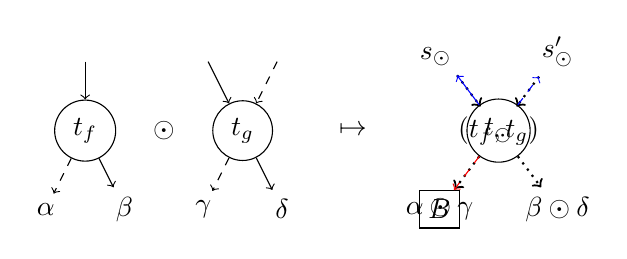
\begin{tikzpicture}
      % 'f'
      \node[shape = circle, draw = black] at (0,0) (f) {$t_f$};

      \node at (-0.5,-1) (f0) {$\alpha$};
      \node at (0.5,-1) (f1) {$\beta$};

      \draw[->, dashed] (f) edge (f0);
      \draw[->]         (f) edge (f1);

      \node at (0,1) (fp) {};
      \draw[->] (fp) edge (f);

      % 'odot'
      \node at (1,0) {$\odot$};

      % 'g'
      \node[shape = circle, draw = black] at (2,0) (g) {$t_g$};

      \node at (1.5,-1) (g0) {$\gamma$};
      \node at (2.5,-1) (g1) {$\delta$};

      \draw[->, dashed] (g) edge (g0);
      \draw[->]         (g) edge (g1);

      \node at (1.5,1) (gp0) {};
      \node at (2.5,1) (gp1) {};
      \draw[->] (gp0) edge (g);
      \draw[->, dashed] (gp1) edge (g);

      \node at (3.4,0) {$\mapsto$};

      % 'f \odot g' (before)
      \node at (4.5,1) (fgp0) {$s_{\odot}\phantom{'}$};
      \node at (6.0,1) (fgp1) {$s_{\odot}'$};

      \onslide<1>{
        \node at (5.25,0) (fg) {$(t_f,t_g)$};

        \draw[->, dotted, thick] (fgp0) edge (fg);
        \draw[->, dotted, thick] (fgp1) edge (fg);
      }

      % 'f \odot g' (after)
      \onslide<2->{
        \node[shape = circle, draw = black] at (5.25,0) (fg) {$t_{\odot}$};

        \draw[blue, ->]         (fg) edge (fgp0);
        \draw[blue, ->, dashed] (fg) edge (fgp1);
      }
      \onslide<3->{
        \node at (6,-1) (fg1) {$\beta \odot \delta$};
        \draw[->, dotted, thick] (fg) edge (fg1);
      }
      \onslide<3>{
        \node at (4.5,-1) (fg0) {$\alpha \odot \gamma$};
        \draw[->, dotted, thick] (fg) edge (fg0);
      }
      \onslide<4>{
        \node[shape=rectangle, draw=black] at (4.5,-1) (fg0) {$\B$};
        \draw[->, red, dashed] (fg) edge (fg0);
      }
    \end{tikzpicture}
  \end{figure}

  \onslide<2->{{\bf Observation (semi-tranposition)}}
  \begin{itemize}
    \onslide<2->{
    \item[{\color{blue} $\leftarrow$} :]{\color{blue} $\arc{s}{}{t}$}\hspace{3pt}
      (Internal Arcs) are output at time $t$ and hence sorted by $t$.
    }

    \onslide<4->{
    \item[{\color{red} $\rightarrow$} :] {\color{red} $\arc{s}{}{\B}$} (Terminal
      Arcs) are output at time $s$.
    }
  \end{itemize}

  \begin{center}
    {\Large \textbf{Time-Forward Processing}}

    Defer resolving products with $Q_{\mathit{app}:1}$, $Q_{\mathit{app}:2}$ :
    \texttt{PriorityQueue}$\langle (\arc{s}{}{(t_f,t_g)}, ...) \rangle$.
  \end{center}
\end{frame}

\begin{frame}[t]
  \frametitle{Apply}

  % priority queues
  \begin{columns}
    \begin{column}{0.46\linewidth}
      $Q_{\mathit{app}:1}$: \texttt{PriorityQueue}$\langle
      (\arc{s}{}{(t_f, t_g)}) \rangle$ sorted on $\min(t_f, t_g)$ in ascending
      order.
    \end{column}
    \begin{column}{0.54\linewidth}
      \onslide<3>{%
        $Q_{\mathit{app}:2}$: \texttt{PriorityQueue}$\langle (\arc{s}{}{(t_f,
          t_g)}, (\alpha, \beta)) \rangle$ sorted on $\max(t_f, t_g)$ in
        ascending order.
      }
    \end{column}
  \end{columns}

  \vspace{10pt}

  % cases
  \begin{columns}[T]
    \begin{column}{0.46\linewidth}
      \textbf{Case 1\phantom{(a)}:}

      $t_f.\mathit{var}() \neq t_g.\mathit{var}()$

      \vspace{10pt}

      \begin{figure}
        \centering

        \begin{tikzpicture}[scale=0.8]
          \node[shape = circle, draw = black] (tf) {$t_f$};

          \node[below left  = 0.5 and 0.2 of tf] (alpha) {$\alpha$};
          \node[below right = 0.5 and 0.2 of tf] (beta)  {$\beta$};

          \node[shape = circle, draw = black, below right=0 and 2.7 of tf] (tg) {$t_g$};

          \node[below left  = 0.5 and 0.2 of tg] (gamma) {$\gamma$};
          \node[below right = 0.5 and 0.2 of tg] (delta) {$\delta$};

          \node[left=2 of tf] (p) {};

          \draw[->, dashed]
            (tf) edge (alpha)
            (tg) edge (gamma)
          ;
          \draw[->]
            (tf) edge (beta)
            (tg) edge (delta)
          ;

          \draw[->, densely dotted, thick]
            (p) edge[bend left] node[above] {$Q_{\mathit{app}:1}$} (tf)
          ;
        \end{tikzpicture}
      \end{figure}
    \end{column}
    \begin{column}{0.54\linewidth}
      \onslide<2->{%
        \textbf{Case 2(a):}

        $t_f.\mathit{var}() = t_g.\mathit{var}() \wedge t_f.\mathit{id}() =
        t_g.\mathit{id}()$
      }

      \vspace{5pt}

      \onslide<3>{%
        \textbf{Case 2(b):}

        $t_f.\mathit{var}() = t_g.\mathit{var}() \wedge t_f.\mathit{id}() \neq
        t_g.\mathit{id}()$

        \begin{figure}
          \centering

          \begin{tikzpicture}[scale=0.8]
            \node[shape = circle, draw = black] (tf) {$t_f$};

            \node[below left  = 0.5 and 0.2 of tf] (alpha) {$\alpha$};
            \node[below right = 0.5 and 0.2 of tf] (beta)  {$\beta$};

            \node[shape = circle, draw = black, right= 2 of tf] (tg) {$t_g$};

            \node[below left  = 0.5 and 0.2 of tg] (gamma) {$\gamma$};
            \node[below right = 0.5 and 0.2 of tg] (delta) {$\delta$};

            \node[left=2 of tf] (p) {};

            \draw[->, dashed]
              (tf) edge (alpha)
              (tg) edge (gamma)
            ;
            \draw[->]
              (tf) edge (beta)
              (tg) edge (delta)
            ;

            \draw[->, densely dotted, thick]
              (p) edge[bend left] node[above] {$Q_{\mathit{app}:1}$} (tf)
              (tf) edge[bend left] node[above] {$Q_{\mathit{app}:2}$} (tg)
            ;
          \end{tikzpicture}
        \end{figure}
      }
    \end{column}
  \end{columns}
\end{frame}

\begin{frame}
  \frametitle{Apply : \emph{Example}}

  % NOTE: The algorithm as presented here has a bug; for more information read
  % the note within the animation file.

  % NOTE: The algorithm as presented here has a bug. Here, we break ties on
% 'min(t1,t2)' with 'max(t1,t2)'. Yet, this can make it unable to merge two
% paths to the same tuple (t1,t2) as intended.
%
% With Adiar v1.0.1 this was fixed by breaking ties with a lexicographical
% sorting of the tuple '(t1,t2)' instead. See the accompanying unit test for a
% counter-example.


\begin{columns}
  \begin{column}{0.24\textwidth}
    \begin{figure}
      \centering

      \begin{subfigure}{1\linewidth}
        \centering

        \begin{tikzpicture}[scale=0.5, every node/.style={transform shape}]
          % nodes
          \node[shape = circle, draw = black]
          (0) {\tiny $(0,0)$};

          \node[shape = circle, draw = black, below right= .3cm and .5cm of 0]
          (1) {\tiny $(1,0)$};

          \node[shape = circle, draw = black, below left=.3cm and .5cm of 1]
          (2) {\tiny $(2,0)$};

          \node[shape = circle, draw = black, below left=.3cm and .5cm of 2]
          (31) {\tiny $(3,0)$};
          \node[shape = circle, draw = black, below right=.3cm and .5cm of 2]
          (32) {\tiny $(3,1)$};

          % leafs
          \node[shape = rectangle, draw = black, below=.4cm of 31]
          (sink_T) {$\top$};

          \node[shape = rectangle, draw = black, below=.4cm of 32]
          (sink_F) {$\bot$};

          % arcs
          \draw[->,dashed]
          (0) edge (2)
          (1) edge (2)
          (2) edge (31)
          (31) edge (sink_T)
          (32) edge (sink_F)
          ;

          \draw[->]
          (0) edge (1)
          (1) edge (32)
          (2) edge (32)
          (31) edge (sink_F)
          (32) edge (sink_T)
          ;

          % animations
          \onslide<2-4>{ % 0
            \node[shape = circle, orange, draw = orange]
            {\tiny $(0,0)$};
            \draw[->,dashed,orange] (0) edge (2);
            \draw[->,orange] (0) edge (1);
          }

          \onslide<5-7>{ % 1
            \node[shape = circle, orange, draw = orange, below right= .3cm and .5cm of 0]
            {\tiny $(1,0)$};
            \draw[->,dashed,orange] (1) edge (2);
            \draw[->,orange] (1) edge (32);
          }

          \onslide<8-12>{ % 2
            \node[shape = circle, orange, draw = orange, below left=.3cm and .5cm of 1]
            {\tiny $(2,0)$};
            \draw[->,dashed,orange] (2) edge (31);
            \draw[->,orange] (2) edge (32);
          }

          \onslide<13-26>{ % 31
            \node[shape = circle, orange, draw = orange, below left=.3cm and .5cm of 2]
            {\tiny $(3,0)$};
            \draw[->,dashed,orange] (31) edge (sink_T);
            \draw[->,orange] (31) edge (sink_F);
          }

          \onslide<27->{ % 32
            \node[shape = circle, orange, draw = orange, below right=.3cm and .5cm of 2]
            {\tiny $(3,1)$};
            \draw[->,dashed,orange] (32) edge (sink_F);
            \draw[->,orange] (32) edge (sink_T);
          }
        \end{tikzpicture}

        \caption{\tiny $(x_0 \wedge x_1 \wedge x_3) \vee (x_2 \oplus x_3)$}
      \end{subfigure}

      \begin{subfigure}{1\linewidth}
        \centering

        \begin{tikzpicture}[scale=0.5, every node/.style={transform shape}]
          % nodes
          \node[shape = circle, draw = black]
          (0) {\tiny $(0,0)$};

          \node[shape = circle, draw = black, below left=1.2cm and .5cm of 0]
          (21) {\tiny $(2,0)$};

          \node[shape = circle, draw = black, below right=1.2cm and .5cm of 0]
          (22) {\tiny $(2,1)$};

          \node[shape = circle, draw = black, below right=0.3cm and .5cm of 21]
          (3) {\tiny $(3,0)$};

          % leafs
          \node[shape = rectangle, draw = black, below right=.4cm and .5cm of 3]
          (sink_F) {$\bot$};

          \node[shape = rectangle, draw = black, below left=.4cm and .5cm of 3]
          (sink_T) {$\top$};

          % arcs
          \draw[->, dashed]
          (0) edge (21)
          (21) edge (sink_T)
          (22) edge (3)
          (3) edge (sink_T)
          ;

          \draw[->]
          (0) edge (22)
          (21) edge (3)
          (22) edge (sink_F)
          (3) edge (sink_F)
          ;

          % animations
          \onslide<2-4>{ % 0
            \node[shape = circle, orange, draw = orange] {\tiny $(0,0)$};
            \draw[->,dashed,orange] (0) edge (21);
            \draw[->,orange] (0) edge (22);
          }

          \onslide<5-12>{ % 21
            \node[shape = circle, orange, draw = orange, below left=1.2cm and .5cm of 0]
            {\tiny $(2,0)$};
            \draw[->,dashed,orange] (21) edge (sink_T);
            \draw[->,orange] (21) edge (3);
          }

          \onslide<13-18>{ % 22
            \node[shape = circle, orange, draw = orange, below right=1.2cm and .5cm of 0]
            {\tiny $(2,1)$};
            \draw[->,dashed,orange] (22) edge (3);
            \draw[->,orange] (22) edge (sink_F);
          }

          \onslide<19->{ % 3
            \node[shape = circle, orange, draw = orange, below right=0.3cm and .5cm of 21]
            {\tiny $(3,0)$};
            \draw[->,dashed,orange] (3) edge (sink_T);
            \draw[->,orange] (3) edge (sink_F);
          }
        \end{tikzpicture}

        \caption{\tiny $\neg (x_0 \ ?\ x_2 \vee x_3 \ :\ x_2 \wedge x_3)$}
      \end{subfigure}
    \end{figure}
  \end{column}
  \begin{column}{0.4\textwidth}
    \centering

    \onslide<4-29>{\tiny Seek:

      \textcolor{orange}{%
        \only<4-7>{$\min((1,0),(2,1))$}%
        \only<8-10>{$\min((2,0),(2,0))$}%
        \only<11-12>{$\min((2,0),(2,1))$}%
        \only<13-15>{$\max((2,0),(2,1))$}%
        \only<16-18>{$\min((3,1),(2,1))$}%
        \only<19-21>{$\min((3,0),(3,0))$}%
        \only<22-23>{$\min((3,1),(3,0))$}%
        \only<24-26>{$\min((3,0),\top)$}%
        \only<27-30>{$\max((3,1),(3,0))$}%
      }
    }
    \vspace{7pt}

    \onslide<3->{ \tiny Priority Queue: $Q_{\mathit{app}:1}$:

      \begin{tabular}{rll}
        [ & \onslide<3-6>{$\arc{(0,0)}{\top}{((1,0),(2,1))}$  & ,}
        \\
          & \onslide<3-9>{$\arc{(0,0)}{\bot}{((2,0),(2,0))}$  & ,}
        \\
          & \onslide<6-11>{$\arc{(1,0)}{\bot}{((2,0),(2,1))}$ & ,}
        \\
          & \onslide<6-17>{$\arc{(1,0)}{\top}{((3,1),(2,1))}$   & ,}
        \\
          & \onslide<14-20>{$\arc{(2,1)}{\bot}{((3,0),(3,0))}$  & ,}
        \\
          & \onslide<9-22>{$\arc{(2,0)}{\top}{((3,1),(3,0))}$   & ,}
        \\
          & \onslide<17-22>{$\arc{(2,2)}{\bot}{((3,1),(3,0))}$  & ,}
        \\
          & \onslide<9-25>{$\arc{(2,0)}{\bot}{((3,0),\top)}$}   & ]
      \end{tabular}
    }

    \vspace{7pt}

    \onslide<12->{ \tiny Priority Queue: $Q_{\mathit{app}:2}$:

      \begin{tabular}{rll}
        [ & \onslide<12-14>{$\arc{(1,0)}{\bot}{((2,0),(2,1))} \quad ((3,0),(3,1))$ & ,}
        \\
          & \onslide<23-28>{$\arc{(2,0)}{\top}{((3,1),(3,0))} \quad (\top,\bot)$ & ,}
        \\
          & \onslide<23-28>{$\arc{(2,2)}{\bot}{((3,1),(3,0))} \quad (\top,\bot)$} & ]
      \end{tabular}
    }

    \vspace{7pt}

  \end{column}
  \begin{column}{0.35\textwidth}
    \centering

    \onslide<7->{ \tiny Output:

      \textcolor{blue}{%
        \only<0-7>{$\arc{(0,0)}{\top}{(1,0)}$}%
        \only<10>{$\arc{(0,0)}{\bot}{(2,0)}$}%
        \only<15>{$\arc{(1,0)}{\bot}{(2,1)}$}%
        \only<18>{$\arc{(1,0)}{\top}{(2,2)}$}%
        \only<21>{$\arc{(2,1)}{\bot}{(3,0)}$}%
        \only<26>{$\arc{(2,0)}{\bot}{(3,1)}$}%
        \only<29>{$\arc{(2,0)}{\top}{(3,2)}, \arc{(2,2)}{\bot}{(3,2)}$}%
      }%
      \textcolor{red}{%
        \only<14>{$\arc{(2,1)}{\top}{\bot}$}%
        \only<17>{$\arc{(2,2)}{\top}{\bot}$}%
        \only<20>{$\arc{(3,0)}{\bot}{\top}, \arc{(3,0)}{\top}{\bot}$}%
        \only<25>{$\arc{(3,1)}{\bot}{\top}, \arc{(3,1)}{\top}{\bot}$}%
        \only<28>{$\arc{(3,2)}{\bot}{\bot}, \arc{(3,2)}{\top}{\bot}$}%
      }%
      {% phantoms
        \only<8-9>{\phantom{$\arc{(0,0)}{\top}{(0,0)}$}}%
        \only<11-13>{\phantom{$\arc{(0,0)}{\top}{(0,0)}$}}%
        \only<16>{\phantom{$\arc{(0,0)}{\top}{(0,0)}$}}%
        \only<19>{\phantom{$\arc{(0,0)}{\top}{(0,0)}$}}%
        \only<22-24>{\phantom{$\arc{(0,0)}{\top}{(0,0)}$}}%
        \only<27>{\phantom{$\arc{(0,0)}{\top}{(0,0)}$}}%
        \only<30>{\phantom{$\arc{(0,0)}{\top}{(0,0)}$}}%
      }%
    }
    \vspace{10pt}

    \begin{tikzpicture}[scale=0.7, every node/.style={transform shape}]
      % level: 0
      % (0,0), (0,0)    1
      \onslide<3->{
        \node[shape = circle, draw = black]
        (00) {\tiny $(0,0)$};
      }

      % level: 1
      % (1,0), (2,1)    1
      \onslide<6->{
        \node[shape = circle, draw = black, below right= .5cm and .3cm of 00]
        (10) {\tiny $(1,0)$};
      }

      % level: 2
      % (2,0), (2,1)    2
      \onslide<14->{
        \node[shape = circle, draw = black, below= 1.4cm of 00]
        (21) {\tiny $(2,1)$};
      }

      % (2,0), (2,0)    1
      \onslide<9->{
        \node[shape = circle, draw = black, left= .7cm of 21]
        (20) {\tiny $(2,0)$};
      }

      % (3,1), (2,1)    3
      \onslide<17->{
        \node[shape = circle, draw = black, right= .7cm of 21]
        (22) {\tiny $(2,2)$};
      }

      % level: 3
      % (3,0), (3,0)    1
      \onslide<20->{
        \node[shape = circle, draw = black, below= .6cm of 20]
        (30) {\tiny $(3,0)$};
      }

      % (3,0), true     2
      \onslide<25->{
        \node[shape = circle, draw = black, below= .6cm of 21]
        (31) {\tiny $(3,1)$};
      }

      % (3,1), (3,0)    3
      \onslide<28->{
        \node[shape = circle, draw = black, below= .6cm of 22]
        (32) {\tiny $(3,2)$};
      }

      % leafs
      \onslide<14->{
        \node[shape = rectangle, draw = black, below right=.9cm and .5cm of 31]
        (sink_F) {$\bot$};
      }

      \onslide<20->{
        \node[shape = rectangle, draw = black, below left=.9cm and .5cm of 31]
        (sink_T) {$\top$};
      }

      % leaf arcs
      \onslide<20->{\draw[->, red, dashed] (30) edge[bend right=10] (sink_T);}
      \onslide<25->{\draw[->, red, dashed] (31) edge[bend right=10] (sink_T);}
      \onslide<28->{\draw[->, red, dashed] (32) edge[bend right=10] (sink_F);}

      \onslide<14->{\draw[->, red] (21) edge[bend left=20] (sink_F);}
      \onslide<17->{\draw[->, red] (22) edge[bend left=60] (sink_F);}
      \onslide<20->{\draw[->, red] (30) edge[bend left=10] (sink_F);}
      \onslide<25->{\draw[->, red] (31) edge[bend left=10] (sink_F);}
      \onslide<28->{\draw[->, red] (32) edge[bend left=10] (sink_F);}
      ;

      % internal arcs
      \onslide<10->{\draw[->, blue, dashed] (20) edge (00);}
      \onslide<15->{\draw[->, blue, dashed] (21) edge (10);}
      \onslide<21->{\draw[->, blue, dashed] (30) edge (21);}
      \onslide<26->{\draw[->, blue, dashed] (31) edge (20);}
      \onslide<29->{\draw[->, blue, dashed] (32) edge (22);}

      \onslide<7->{\draw[->, blue] (10) edge (00);}
      \onslide<18->{\draw[->, blue] (22) edge (10);}
      \onslide<29->{\draw[->, blue] (32) edge (20);}
    \end{tikzpicture}

    \begin{center}
      {\bf \footnotesize (c)} ~ $(a) \land (b)$
    \end{center}
  \end{column}
\end{columns}

\end{frame}

\begin{frame}
  \frametitle{Apply}

  \setvalue{tandem_apply  = lightgray}
  \setvalue{tandem_reduce = black}

  \begin{figure}[ht!]
  \centering
  \begin{tikzpicture}[every text node part/.style={align=center}]
    % Boxes
    \draw[color=\getvalue{tandem_apply}]
      (0,0) rectangle ++(2,1)
      node[pos=.5]{\texttt{Apply}}
    ;
    \draw[color=\getvalue{tandem_reduce}]
      (5,0) rectangle ++(2,1)
      node[pos=.5]{\texttt{Reduce}}
    ;

    % Arcs
    \draw[->, color=\getvalue{tandem_apply}]
      (-0.5,0.8) -- ++(0.5,0)
      node[pos=-1.6]{$f$ \texttt{nodes}}
    ;
    \draw[->, color=\getvalue{tandem_apply}]
      (-0.5,0.2) -- ++(0.5,0)
      node[pos=-1.6]{$g$ \texttt{nodes}}
    ;

    \draw[blue, ->] (2,0.8) -- ++(3,0)
      node[pos=0.5,above]
      {\small\color{blue} internal \texttt{arcs}}
    ;

    \node at (3.5,0.5) {\textcolor{darkgray}{$f \odot g$ \texttt{arcs}}};

    \draw[red, ->] (2,0.2) -- ++(3,0) node[pos=0.5,below]{\small\color{red} leaf
      \texttt{arcs}};

    \draw[->, color=\getvalue{tandem_reduce}]
      (7,0.5) -- ++(0.5,0)
      node[pos=3.2]{$f \odot g$ \texttt{nodes}}
    ;
  \end{tikzpicture}
\end{figure}
\end{frame}

\begin{frame}
  \frametitle{Apply (Reduce)}

  \begin{figure}
    \centering

    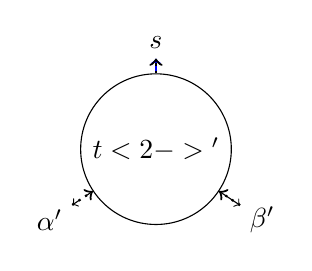
\begin{tikzpicture}[scale=0.9]
      \node[shape = circle, draw = black] at (0,0) (t) {$t\onslide<2->{'}$};

      \node at (-1.5,-1) (t0) {$\alpha'$};
      \node at ( 1.5,-1) (t1) {$\beta'$};

      \node at ( 0, 1.5) (s) {$s$};

      \onslide<1>{
        \draw[->, dotted, thick]
          (t0) edge (t)
          (t1) edge (t)
        ;
      }
      \onslide<1-2>{
        \draw[blue, ->] (t) edge (s);
      }
      \onslide<2->{
        \draw[->, dashed] (t) edge (t0);
        \draw[->]         (t) edge (t1);
      }
      \onslide<3->{
        \draw[->, dotted, thick] (t) edge (s);
      }
    \end{tikzpicture}
  \end{figure}

  \begin{center}
    {\Large \textbf{Time-Forward Processing}}

    Send reduction $t'$ with $Q_{\mathit{red}}$ : \texttt{PriorityQueue}$\langle
    (\arc{s}{}{t'}) \rangle$ descending on parent $s$.
  \end{center}

  \onslide<3->{{\bf Observation (semi-tranposition)}}
  \begin{itemize}
    \onslide<3->{
    \item[{\color{blue} $\leftarrow$} :]{\color{blue} $\arc{s}{}{t}$}\hspace{3pt}
      (Internal Arcs) provide parents of unreduced node $t$.
    }

    \onslide<4->{
    \item[{\color{red} $\rightarrow$} :] {\color{red} $\arc{s}{}{\B}$} (Terminal
      Arcs) are reduced and already sorted as per $Q_{\mathit{red}}$.
    }
  \end{itemize}
\end{frame}

\begin{frame}
  \frametitle{Apply (Reduce)}

    \begin{figure}
    \centering

    \begin{tikzpicture}[scale=0.8]
      % reduction rule 2
      \node at (0,2) (s1) {};
      \onslide<-4>{
        \node[shape=circle, draw=black] at (0,0) (t1) {$x_i$};

        \node[below left  = 0.7 and 0.2 of t1] (t1_0) {$\alpha'$};
        \node[below right = 0.7 and 0.2 of t1] (t1_1) {$\beta'$};
      }
      \onslide<5->{
        \node[shape=circle, draw=gray, color=gray] at (0,0) (t1) {$x_i$};

        \node[color=gray, below left  = 0.7 and 0.2 of t1] (t1_0) {$\alpha'$};
        \node[color=gray, below right = 0.7 and 0.2 of t1] (t1_1) {$\beta'$};
      }

      \node at (4,2) (s2) {};
      \only<1-3,6->{
        \node[shape = circle, draw = black] at (4,0) (t2) {$x_i$};
      }
      \only<4-5>{
        \node[shape = circle, draw = black] at (8,0) (t2) {$x_i$};
      }

      \node[below left  = 0.7 and 0.2 of t2] (t2_0) {$\gamma'$};
      \node[below right = 0.7 and 0.2 of t2] (t2_1) {$\delta'$};

      \node at (8,2) (s3) {};
      \only<1-3,6->{
        \node[shape = circle, draw = black] at (8,0) (t3) {$x_i$};
      }
      \only<4-5>{
        \node[shape = circle, draw = black] at (4,0) (t3) {$x_i$};
      }

      \node[below left  = 0.7 and 0.2 of t3] (t3_0) {$\alpha'$};
      \node[below right = 0.7 and 0.2 of t3] (t3_1) {$\beta'$};

      % -- priority queue
      \only<1-2>{
        \draw[->, dotted, thick]
          (t1_0) edge (t1)
          (t1_1) edge (t1)
          (t2_0) edge (t2)
          (t2_1) edge (t2)
          (t3_0) edge (t3)
          (t3_1) edge (t3)
        ;
      }
      \only<7>{
        \draw[->, dotted, thick]
          (t3) edge (s1)
          (t2) edge[bend right=40] (s2)
          (t3) edge[bend right=40] (s3)
        ;
      }

      % -- children edges
      \only<3->{
        \draw[->, dashed]
          (t2) edge (t2_0)
          (t3) edge (t3_0)
        ;
        \draw[->]
          (t2) edge (t2_1)
          (t3) edge (t3_1)
        ;
        \only<-4>{
          \draw[->, dashed] (t1) edge (t1_0);
          \draw[->]         (t1) edge (t1_1);
        }
        \only<5->{
          \draw[gray, ->, dashed] (t1) edge (t1_0);
          \draw[gray, ->]         (t1) edge (t1_1);
        }
      }

      % -- mapping
      \only<5>{
        \draw[purple, |->, thick, dotted] (t1) edge[bend right=20] (t3);
      }
      \only<6->{
        \draw[purple, |->, thick, dotted] (t1) edge[bend right=20] (t3);
      }

      % -- parent pointers
      \only<1-3,6->{
        \draw[blue, ->]
          (t1) edge (s1)
          (t2) edge (s2)
          (t3) edge (s3)
        ;
      }
      \only<4-5>{
        \draw[blue!50!white, ->, dotted]
          (t1) edge (s1)
          (t2) edge (s2)
          (t3) edge (s3)
        ;
      }

      % reduction rule 1
      \node at (12,2) (s0) {};

      \node at (12,-1.53) (t0_0) {$\alpha'$};

      % -- before
      \onslide<1>{
        \node[shape=circle, draw=black] at (12,0) (t0) {$x_i$};
      }

      % -- after
      \onslide<2->{
        \node[shape=circle, draw=gray, color=gray] at (12,0) (t0) {$x_i$};
        \draw[purple, |->, thick, dotted] (t0) edge (t0_0);
      }

      % -- priority queue
      \onslide<1>{
        \draw[->, dotted, thick] (t0_0) edge[bend left]  (t0);
        \draw[->, dotted, thick] (t0_0) edge[bend right] (t0);
      }
      \onslide<7->{
        \draw[->, dotted, thick] (t0_0) edge[bend right=40] (s0);
      }
      \draw[blue,->] (t0) edge (s0);
    \end{tikzpicture}
  \end{figure}

  \textbf{Reduce Level $i$}:
  \begin{enumerate}
    \onslide<1->{%
    \item Obtain nodes from $Q_{\mathit{red}}$ and {\color{red} terminal
        arcs}. Filter and {\color{purple} remember} redundant nodes.
    }%
    \onslide<4->{%
    \item Sort remaining nodes by children, output unique nodes, and
      {\color{purple} remember} duplications.
    }%
    \onslide<6->{%
    \item Sort back to match {\color{blue} internal arcs} and forward to parents
      with $Q_{\mathit{red}}$.
    }%
  \end{enumerate}
\end{frame}

\begin{frame}
  \frametitle{Apply (Reduce) : \emph{Example}}

  \begin{columns}
  \begin{column}{0.25\linewidth}
    \centering

    \begin{tikzpicture}[scale=0.7, every node/.style={transform shape}]
      % level: 0
      % (0,0), (0,0)    1
      \node[shape = circle, draw = black]
      (00) {\tiny $(0,0)$};

      % level: 1
      % (1,0), (2,1)    1
      \node[shape = circle, draw = black, below right= .5cm and .3cm of 00]
      (10) {\tiny $(1,0)$};

      % level: 2
      % (2,0), (2,1)    2
      \node[shape = circle, draw = black, below= 1.4cm of 00]
      (21) {\tiny $(2,1)$};

      % (2,0), (2,0)    1
      \node[shape = circle, draw = black, left= .7cm of 21]
      (20) {\tiny $(2,0)$};

      % (3,1), (2,1)    3
      \node[shape = circle, draw = black, right= .7cm of 21]
      (22) {\tiny $(2,2)$};

      % level: 3
      % (3,0), (3,0)    1
      \node[shape = circle, draw = black, below= .6cm of 20]
      (30) {\tiny $(3,0)$};

      % (3,0), true     2
      \node[shape = circle, draw = black, below= .6cm of 21]
      (31) {\tiny $(3,1)$};

      % (3,1), (3,0)    3
      \node[shape = circle, draw = black, below= .6cm of 22]
      (32) {\tiny $(3,2)$};

      % leafs
      \node[shape = rectangle, draw = black, below right=.9cm and .5cm of 31]
      (sink_F) {$\bot$};

      \node[shape = rectangle, draw = black, below left=.9cm and .5cm of 31]
      (sink_T) {$\top$};

      % leaf arcs
      \draw[->, red, dashed]
      (30) edge[bend right=10] (sink_T)
      (31) edge[bend right=10] (sink_T)
      (32) edge[bend right=10] (sink_F)
      ;

      \draw[->, red]
      (21) edge[bend left=20] (sink_F)
      (22) edge[bend left=60] (sink_F)
      (30) edge[bend left=10] (sink_F)
      (31) edge[bend left=10] (sink_F)
      (32) edge[bend left=10] (sink_F)
      ;

      % internal arcs
      \draw[->, blue, dashed]
      (20) edge (00)
      (21) edge (10)
      (30) edge (21)
      (31) edge (20)
      (32) edge (22)
      ;

      \draw[->, blue]
      (10) edge (00)
      (22) edge (10)
      (32) edge (20)
      ;

      % animations
      \onslide<2>{
        \draw[->, orange, dashed, thick] (32) edge[bend right=10] (sink_F);
        \draw[->, orange, thick] (32) edge[bend left=10] (sink_F);
      }
      \onslide<3>{
        \draw[->, orange, dashed, thick] (31) edge[bend right=10] (sink_T);
        \draw[->, orange, thick] (31) edge[bend left=10] (sink_F);
      }
      \onslide<4>{
        \draw[->, orange, dashed, thick] (30) edge[bend right=10] (sink_T);
        \draw[->, orange, thick, thick] (30) edge[bend left=10] (sink_F);
      }
      \onslide<7>{
        \draw[->, purple, dashed, thick] (32) edge (22);
        \draw[->, purple, thick] (32) edge (20);
      }
      \onslide<8>{
        \draw[->, purple, dashed, thick] (31) edge (20);
      }
      \onslide<9>{
        \draw[->, purple, dashed, thick] (30) edge (21);
      }
      \onslide<10>{
        \draw[->, orange, thick] (22) edge[bend left=60] (sink_F);
      }
      \onslide<11>{
        \draw[->, orange, thick] (21) edge[bend left=20] (sink_F);
      }
      \onslide<15>{
        \draw[->, purple, thick] (22) edge (10);
      }
      \onslide<16>{
        \draw[->, purple, dashed, thick] (21) edge (10);
      }
      \onslide<17>{
        \draw[->, purple, dashed, thick] (20) edge (00);
      }
      \onslide<20>{
        \draw[->, purple, thick] (10) edge (00);
      }
    \end{tikzpicture}

    \begin{center}
      {\bf \footnotesize (c)} ~ $(a) \land (b)$
    \end{center}
  \end{column}
  \begin{column}{0.49\linewidth}
    \centering

    \onslide<7->{ \tiny Priority Queue: $Q_{\mathit{red}}$:

      \begin{tabular}{rll}
        [ & \onslide<7-9>{$\arc{(2,2)}{\bot}{\bot}$      & ,}
        \\
          & \onslide<9-10>{$\arc{(2,1)}{\bot}{(3,\max)}$ & ,}
        \\
          & \onslide<7-11>{$\arc{(2,0)}{\top}{\bot}$     & ,}
        \\
          & \onslide<8-11>{$\arc{(2,0)}{\bot}{(3,\max)}$ & ,}
        \\
          & \onslide<15-17>{$\arc{(1,0)}{\top}{\bot}$      & ,}
        \\
          & \onslide<16-17>{$\arc{(1,0)}{\bot}{(2,\max)}$  & ,}
        \\
          & \onslide<20>{$\arc{(0,0)}{\top}{(1,\max)}$  & ,}
        \\
          & \onslide<17-20>{$\arc{(0,0)}{\bot}{(2,\max)}$} & ]
      \end{tabular}
    }

    \vspace{10pt}

    \only<2-9>{ \tiny Level: $3$

      \only<2->{
        \begin{tabular}{r>{\centering}m{3cm}l}
          [ & \onslide<2-6>{$[(3,2) \mapsto \bot]$} & ]
        \end{tabular}
      }

      \vspace{5pt}

      \onslide<3->{%
        \begin{tabular}{r>{\centering}m{3cm}l}
          [ & \only<3-4>{$\triple{(3,1)}{\top}{\bot}$}
              \only<5-7>{$[(3,1) \mapsto (3,\max)]$}
              \only<8->{\phantom{$[(3,1) \mapsto (3,\max)]$}}
          & ,
          \\
            & \only<4-5>{$\triple{(3,0)}{\top}{\bot}$}
              \only<6-8>{$[(3,0) \mapsto (3,\max)]$}
          & ]
        \end{tabular}
      }%
    }
    \only<10-17>{ \tiny Level: $2$

      \only<10->{
        \begin{tabular}{r>{\centering}m{3cm}l}
          [ & \onslide<10-14>{$[(2,2) \mapsto \bot]$} & ]
        \end{tabular}
      }

      \vspace{5pt}

      \onslide<11->{%
        \begin{tabular}{r>{\centering}m{3cm}l}
          [ & \only<11-12>{$\triple{(2,1)}{(3,\max)}{\bot}$}
              \only<13-15>{$[(2,1) \mapsto (2,\max)]$}
              \only<16->{\phantom{$[(2,1) \mapsto (2,\max)]$}}
          & ,
          \\
            & \only<12-13>{$\triple{(2,0)}{(3,\max)}{\bot}$}
              \only<14-16>{$[(2,0) \mapsto (2,\max)]$}
          & ]
        \end{tabular}
      }%
    }
    \only<18-20>{ \tiny Level: $1$

      \begin{tabular}{r>{\centering}m{3cm}l}
        [ & \phantom{$[(1,0) \mapsto \bot]$} & ]
      \end{tabular}

      \vspace{5pt}

      \begin{tabular}{r>{\centering}m{3cm}l}
        [ & \only<18>{$\triple{(1,0)}{(2,\max)}{\bot}$}
            \only<19>{$[(1,0) \mapsto (1,\max)]$}
            \only<20->{\phantom{$[(1,0) \mapsto (1,\max)]$}}
        & ]
      \end{tabular}
      \vspace{8pt}
    }
    \only<21-23>{ \tiny Level: $0$

      \begin{tabular}{r>{\centering}m{3cm}l}
        [ & \phantom{$[(1,0) \mapsto \bot]$} & ]
      \end{tabular}

      \vspace{5pt}

      \begin{tabular}{r>{\centering}m{3cm}l}
        [ & \only<21>{$\triple{(0,0)}{(2,\max)}{(1,\max)}$}
            \only<22>{$[(0,0) \mapsto (0,\max)]$}
            \only<23->{\phantom{$[(0,0) \mapsto (1,\max)]$}}
        & ]
      \end{tabular}
      \vspace{8pt}
    }

  \end{column}
  \begin{column}{0.25\linewidth}
    \centering

    \onslide<5->{ \tiny Output:

      {%
        \only<5>{$\triple{(3,\max)}{\top}{\bot}$}%
        \only<13>{$\triple{(2,\max)}{(3,\max)}{\bot}$}%
        \only<19>{$\triple{(1,\max)}{(2,\max)}{\bot}$}%
        \only<22>{$\triple{(0,\max)}{(2,\max)}{(1,\max)}$}%
      }%
      {% phantoms
        \only<-4>{\phantom{$\triple{(3,0)}{\bot}{\top}$}}%
        \only<6-12>{\phantom{$\triple{(3,0)}{\bot}{\top}$}}%
        \only<14-18>{\phantom{$\triple{(3,0)}{\bot}{\top}$}}%
        \only<20-21>{\phantom{$\triple{(3,0)}{\bot}{\top}$}}%
        \only<23->{\phantom{$\triple{(3,0)}{\bot}{\top}$}}%
      }%
    }
    \vspace{10pt}

    \begin{tikzpicture}[scale=0.7, every node/.style={transform shape}]
      % nodes
      \onslide<22->{
        \node[shape = circle, draw = black]
        (0) {\tiny $(0,\max)$};
      }

      \onslide<19->{
        \node[shape = circle, draw = black, below right= .3cm and .5cm of 0]
        (1) {\tiny $(1,\max)$};
      }

      \onslide<13->{
        \node[shape = circle, draw = black, below left=.3cm and .5cm of 1]
        (2) {\tiny $(2,\max)$};
      }

      \onslide<5->{
        \node[shape = circle, draw = black, below=.4cm of 2]
        (3) {\tiny $(3,\max)$};
      }

      \onslide<5->{
        \node[shape = rectangle, draw = black, below right=.5cm and .5cm of 3]
        (sink_F) {$\bot$};
      }

      \onslide<5->{
        \node[shape = rectangle, draw = black, below left=.5cm and .5cm of 3]
        (sink_T) {$\top$};
      }

      \onslide<5->{\draw[->, dashed] (3) edge (sink_T);}
      \onslide<13->{\draw[->, dashed] (2) edge (3);}
      \onslide<19->{\draw[->, dashed] (1) edge (2);}
      \onslide<22->{\draw[->, dashed] (0) edge (2);}

      \onslide<5->{\draw[->] (3) edge (sink_F);}
      \onslide<13->{\draw[->] (2) edge[bend left=6] (sink_F);}
      \onslide<19->{\draw[->] (1) edge (sink_F);}
      \onslide<22->{\draw[->] (0) edge (1);}
    \end{tikzpicture}

    \begin{center}
      {\bf \footnotesize (d)} ~ $(a) \land (b)$ reduced
    \end{center}
  \end{column}
\end{columns}

\end{frame}

\begin{frame}
  \begin{table}
    \centering
    \begin{tabular}{rl}
      Algorithm                 & I/O-Complexity
      \\ \hline \hline
      \lstinline{bdd_pathcount} & $O(\sort(N_f))$
      \\ \hline
      \lstinline{bdd_not}       & $2 N_f / B$
      \\
      \lstinline{bdd_restrict}  & $O(\sort(N_f))$
      \\
      \lstinline{bdd_apply}     & $O(\sort(N_f \cdot N_g))$
    \end{tabular}
  \end{table}
\end{frame}

\begin{frame}
  \begin{figure}
    \centering

    \begin{tikzpicture}
      \begin{axis}[%
        width=0.70\linewidth, height=0.42\linewidth,
        every tick label/.append style={font=\scriptsize},
        % x-axis
        xlabel={number of BDD nodes},
        xmajorgrids=true,
        xmin=51000000,
        xmax=300000000000,
        xmode = log,
        % y-axis
        ymin=0,
        ymax=2.2,
        ytick distance={0.5},
        ylabel={$\mu$s / BDD node},
        yminorgrids=true,
        ymajorgrids=true,
        grid style={dashed,black!20},
        ]

        \only<1-> {
          \addplot+ [style=plot_buddy]
          table {./data/queens_buddy_time_per_node.tex};
        }
        \only<1-> {
          \addplot+ [style=plot_cudd]
          table {./data/queens_cudd_time_per_node.tex};
        }
        \only<1-> {
          \addplot+ [style=plot_sylvan]
          table {./data/queens_sylvan_time_per_node.tex};
        }

        \only<2-> {
          \addplot+ [style=plot_adiar]
          table {./data/queens_adiar_time_per_node.tex};
        }
      \end{axis}

    \end{tikzpicture}

    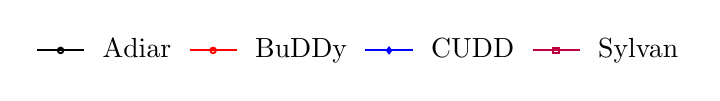
\begin{tikzpicture}
      \begin{customlegend}[
        legend columns=-1,
        legend style={draw=none,column sep=1ex},
        legend entries={Adiar, BuDDy, CUDD, Sylvan}
        ]
        \addlegendimage{style=plot_adiar}
        \addlegendimage{style=plot_buddy}
        \addlegendimage{style=plot_cudd}
        \addlegendimage{style=plot_sylvan}
      \end{customlegend}
    \end{tikzpicture}

    \caption{Running time for the \emph{N-Queens} problems.}
  \end{figure}
\end{frame}

\subsection{Equality Checking}

\begin{frame}[plain,noframenumbering]{}
  \frametitle{Contents}
  \tableofcontents[currentsection, currentsubsection]
\end{frame}

\begin{frame}
  \begin{table}
    \centering
    \begin{tabular}{rl}
      Algorithm                 & I/O-Complexity
      \\ \hline \hline
      \lstinline{bdd_pathcount} & $O(\sort(N_f))$
      \\ \hline
      \lstinline{bdd_not}       & $2 N_f / B$
      \\
      \lstinline{bdd_restrict}  & $O(\sort(N_f))$
      \\
      \lstinline{bdd_apply}     & $O(\sort(N_f \cdot N_g))$
                                  \pause
      \\ \hline
      \lstinline{bdd_equal}     & ?
    \end{tabular}
  \end{table}
\end{frame}

\begin{frame}
  \frametitle{Equality Checking}

  \vspace{30pt}
  \begin{center}
    {\huge $f \leftrightarrow g \equiv \top$}
  \end{center}

  \pause
  \vspace{20pt}

  \begin{equation*}
    \underbrace{O(\sort(N^2))}_{\texttt{Apply}}
    + \underbrace{O(\sort(N^2))}_{\texttt{Reduce}}
    + \underbrace{O(1))}_{\text{check is } \top}
    = O(\sort(N^2))
  \end{equation*}
\end{frame}

\begin{frame}[t]
  \frametitle{Equality Checking}

  \begin{theorem}[Bryant '86]
    Let $\pi$ be a variable order and $f : \B^n \rightarrow \B$ then there
    exists a unique (up to isomorphism) Reduced Ordered Binary Decision
    Diagram representing $f$ with ordering $\pi$.
  \end{theorem}

  \pause
  {\bf Trivial cases: $f \not \equiv g$ if there is a mismatch in}

  \begin{tabular}{c l l l}
    {\tiny $\blacksquare$} & $N_f \neq N_g$       & Number of nodes            & $O(1)$ I/Os
    \\
    {\tiny $\blacksquare$} & $L_f \neq L_g$       & Number of levels           & $O(1)$ I/Os
    \\
    {\tiny $\blacksquare$} & $N_{f,i} \neq N_{g,i}$ & Number of nodes on a level & $O(L/B)$ I/Os
    \\
    {\tiny $\blacksquare$} & $L_{f,i} \neq L_{g,i}$ & Label of an $i$th level    & $O(L/B)$ I/Os
  \end{tabular}
\end{frame}

\begin{frame}[t]
  \frametitle{Equality Checking}

  % TODO: code duplication
  \begin{theorem}[Bryant '86]
    Let $\pi$ be a variable order and $f : \B^n \rightarrow \B$ then there
    exists a unique (up to isomorphism) Reduced Ordered Binary Decision
    Diagram representing $f$ with ordering $\pi$.
  \end{theorem}

  \begin{figure}
    \centering

    \begin{tikzpicture}[scale=1, every node/.style={transform shape}]
      % f
\node[shape = circle, black, draw = black] (i1)
{$x_i$};

\onslide<3->{
  \node[shape = rectangle, draw = black, below left=1.2cm and 0.4cm of i1] (child1_1)
  { $\top$ };
}
\onslide<1-2>{
  \node[shape = circle, draw = black, below left=1.2cm and 0.4cm of i1] (child1_1)
  { \phantom{$x_j$} };
}

\node[shape = circle, draw = black, below right=1.2cm and 0.4cm of i1] (child1_2)
{
  \only<1>{\phantom{$x_j$}}%
  \only<2->{$x_j$}%
};

\draw[->, dashed] (i1) edge (child1_1);
\draw[->] (i1) edge (child1_2);

% g
\node[shape = circle, black, draw = black, right=5cm of i1] (i2) {$x_i$};

\onslide<3->{
  \node[shape = rectangle, draw = black, below left=1.2cm and 0.4cm of i2] (child2_1)
  {
    \only<1-3,5->{$\top$}%
    \only<4>{$\bot$}%
  };
}
\onslide<1-2>{
  \node[shape = circle, draw = black, below left=1.2cm and 0.4cm of i2] (child2_1)
  { \phantom{$x_j$}};
}

\onslide<6->{
  \node[shape = rectangle, draw = black, below right=1.2cm and 0.4cm of i2] (child2_2)
  { $\top$ };
}
\onslide<1-5>{
\node[shape = circle, draw = black, below right=1.2cm and 0.4cm of i2] (child2_2)
{
  \only<1>{\phantom{$x_j$}}%
  \only<2-4>{$x_j$}%
  \only<5->{$x_k$}%
};
}

\draw[->, dashed] (i2) edge (child2_1);
\draw[->] (i2) edge (child2_2);

% isomorphism
\onslide<1-3>{
  \draw[blue, densely dashed, thick] (i1) edge (i2);
}

\node[shape = circle, black,below right=0.3cm and 2.3cm of i1] {$\Updownarrow$};

\onslide<1-3,5->{
  \draw[white!40!blue, densely dashed, thick](child1_1) edge[bend right=50] (child2_1);
}

\onslide<1-4>{
  \draw[black!40!blue, densely dashed, thick] (child1_2) edge[bend right=50] (child2_2);
}


    \end{tikzpicture}
  \end{figure}

\end{frame}

\begin{frame}[t]
  \frametitle{Equality Checking}

  % TODO: code duplication
  \begin{theorem}[Bryant '86]
    Let $\pi$ be a variable order and $f : \B^n \rightarrow \B$ then there
    exists a unique (up to isomorphism) Reduced Ordered Binary Decision
    Diagram representing $f$ with ordering $\pi$.
  \end{theorem}

  \texttt{IsIsomorphic($f$, $g$)}
  \begin{itemize}
  \item Check whether root $v_f$ of $f$ and root $v_g$ of $g$ have a local violation.
  \item Check $\mathit{low}(v_f) \sim \mathit{low}(v_g)$ and $\mathit{high}(v_f)
    \sim \mathit{high}(v_g)$ ``recursively''.
  \end{itemize}
  Return \texttt{false} on first violation. If there are no violations then return \texttt{true}.
  \pause
  \begin{equation*}
    \underbrace{O(\sort(N^2))}_{\texttt{Apply}'}
    + \underbrace{\hcancel[gray]{O(\sort(N^2))}}_{\texttt{Reduce}}
    + \underbrace{\hcancel[gray]{O(1))}}_{\text{check is } \top}
    =
    O(\sort(N^2))
  \end{equation*}
\end{frame}

\begin{frame}[t]
  \frametitle{Equality Checking}

  % TODO: code duplication
  \begin{theorem}[Bryant '86]
    Let $\pi$ be a variable order and $f : \B^n \rightarrow \B$ then there
    exists a unique (up to isomorphism) Reduced Ordered Binary Decision
    Diagram representing $f$ with ordering $\pi$.
  \end{theorem}

  \vspace{-10pt}
  \begin{figure}
    \centering

    \begin{tikzpicture}[scale=0.9, every node/.style={transform shape}]
      % f
\node[shape = circle, black, draw = black] (f1) {\tiny $x_i$};
\node[shape = circle, black, draw = black, right =of f1] (f2) {\tiny $x_i$};
\node[right =of f2] (f_dots) {$\dots$};
\node[shape = circle, black, draw = black, right =of f_dots] (fn) {\tiny $x_i$};

\draw [
thick,
decoration={
  brace,
  mirror,
  raise=0.5cm
},
decorate
] (-0.25,-0.1) -- ++(5.5,0)
node [pos=0.5,anchor=north,yshift=-0.55cm] {$N_{f,i}$};

% g

\node[shape = circle, black, draw = black, right =2cm of fn] (g1) {\tiny $x_i$};
\node[shape = circle, black, draw = black, right =of g1] (g2) {\tiny $x_i$};
\node[right =of g2] (g_dots) {$\dots$};
\node[shape = circle, black, draw = black, right =of g_dots] (gn) {\tiny $x_i$};

\draw [
thick,
decoration={
  brace,
  mirror,
  raise=0.5cm
},
decorate
] (7.3,-0.1) -- ++(5.5,0)
node [pos=0.5,anchor=north,yshift=-0.55cm] {$N_{g,i}$};

% isomorphism
\draw[blue, densely dashed]
  (f1) edge[bend left=20] (g2)
  (f2) edge[bend left=20] (g_dots)
  (f_dots) edge[bend left=20] (g1)
  (f_dots) edge[bend left=20] (gn)
  (fn) edge[bend left=20] (g_dots)
;
    \end{tikzpicture}
  \end{figure}
  \pause
  \vspace{-20pt}
  Return \texttt{false} if more than $N_{f,i} = N_{g,i}$ pairs of nodes are checked on level $i$.
  \begin{equation*}
    \underbrace{O (\sort (\Sigma_{i}\ N_{f,i} ) )}_{\texttt{Apply}''}
    =
    O(\sort(N))
  \end{equation*}
\end{frame}

\begin{frame}
  \frametitle{Equality Checking}

  \begin{center}
  \begin{tikzpicture}
    % i, max
    \onslide<2->{
      \node[shape = rectangle, draw = black, minimum width=84, rounded corners=5]
      (0) {\small $i$, $\text{max}$};

      \node[shape = circle, draw = black, minimum width=24, below left =1 and -1 of 0]
      (00) {$\beta$};
      \draw[->,dashed] (0) edge[bend right=15] (00);

      \node[shape = circle, draw = black, minimum width=24, below right=1 and -1 of 0]
      (01) {$\alpha$};
      \draw[->] (0) edge[bend left=15] (01);
    }

    % i, max-1
    \onslide<3->{
      \node[shape = rectangle, draw = black, minimum width=84, rounded corners=5, left =of 0]
      (1) {\small $i$, $\text{max}-1$};

      \node[shape = circle, draw = black, minimum width=24, below left =1 and -1 of 1]
      (10) {$\delta$};
      \draw[->,dashed] (1) edge[bend right=15] (10);

      \node[shape = circle, draw = black, minimum width=24, below right=1 and -1 of 1]
      (11) {$\gamma$};
      \draw[->] (1) edge[bend left=15] (11);
    }

    % ...
    \onslide<3->{
      \node[left =of 1] (dots1) { \dots};
    }

    % i, max-N+1
    \onslide<4->{
      \node[shape = rectangle, draw = black, minimum width=84, rounded corners=5, left =of dots1]
      (n) {\small $i$, $\text{max}-N_{f,i}+1$};

      \node[shape = circle, draw = black, minimum width=24, below left =1 and -1 of n]
      (n0) {$\zeta$};
      \draw[->,dashed] (n) edge[bend right=15] (n0);

      \node[shape = circle, draw = black, minimum width=24, below right=1 and -1 of n]
      (n1) {$\epsilon$};
      \draw[->] (n) edge[bend left=15] (n1);
    }

    % < ... < <
    \onslide<5->{
      \node[below left= 1.05 and 0.3 of 0] (comp0)     {{\bf <}};
    }
    \onslide<6->{
      \node[below left= 1.05 and 0.3 of 1]  (comp1)    {{\bf <}};
      \node[below left =1.20 and 1.0 of 1]  (compdots) {\dots};
      \node[below right=1.05 and 0.22 of n] (compn)    {{\bf <}};
    }
  \end{tikzpicture}
\end{center}

  {\bf Observation}

  \vspace{-10pt}
  Each level output by the \texttt{Reduce} algorithm has the following properties:
  \begin{itemize}
    \onslide<4->{
    \item Nodes on level $i$ have their identifiers \emph{consecutively} numbered.
    }
    \onslide<6->{
    \item Nodes on level $i$ are output sorted by their children.
    }
  \end{itemize}
\end{frame}

\begin{frame}
  \frametitle{Equality Checking}

  \begin{theorem}
    If $G_f$ and $G_g$ are outputs of \lstinline{Reduce}.
    \begin{center}
      $G_f \sim G_g$ $\iff$ For all $i \in [0; N_f)$ the node $G_f[i]$ matches
      $G_g[i]$ numerically.
    \end{center}
  \end{theorem}
  \begin{proof}
    $\Leftarrow$ : Must describe the exact same graph.

    $\Rightarrow$ : Strong induction on BDD levels bottom-up.
  \end{proof}

  \pause
  \begin{corollary}
    If $G_f$ and $G_g$ are outputs of \lstinline{Reduce} then $f \equiv g$ is
    computable using $2 \cdot N/B$ I/Os.
  \end{corollary}
\end{frame}


\begin{frame}
  \frametitle{Equality Checking}

  \begin{table}
    \centering
    \begin{tabular}{r | l}
      Algorithm                         & Time (s)
      \\ \hline
      $f \leftrightarrow g \equiv \top$ & 0.38
      \\ \onslide<2->{
      $O(\sort(N))$                     & 0.058}
      \\ \onslide<3->{
      $2N/B$                            & 0.006}
    \end{tabular}

    \caption{Checking the (EPFL Benchmark) \emph{voter} circuit's single output
      gate ($\abs{N_f} = \abs{N_g} = 5.76~\text{MiB}$).}
  \end{table}
\end{frame}

\blankframe

\begin{frame}[plain,noframenumbering]
  % custom copy of fram/endslate.tex
  {\Large \textbf{Steffan Christ Sølvsten}}
  \begin{columns}
    \begin{column}{0.4\linewidth}
      \vspace{1pt} {\hrule width\linewidth}

      \vspace{5pt}

      \begin{itemize}
      \item[\faIcon{envelope}] \mailto{soelvsten@cs.au.dk}
      \item[\faIcon{globe}] \href{https://ssoelvsten.github.io}{ssoelvsten.github.io}
      \end{itemize}

      \vspace{10pt}

      {\Large \textbf{Adiar}}
      \vspace{1pt} {\hrule width\linewidth}

      \vspace{5pt}

      \begin{itemize}
      \item[\faIcon{code}]
        \href{http://github.com/ssoelvsten/adiar}{github.com/ssoelvsten/adiar}
      \item[\faIcon{book}\hspace{2pt}]
        \href{http://ssoelvsten.github.io/adiar}{ssoelvsten.github.io/adiar}
      \end{itemize}

      \vspace{10pt}

      
\includegraphics[width=0.5\linewidth]{external/aulogo_uk_var2_black.eps}
    \end{column}
    \begin{column}{0.6\linewidth}
      \begin{table}
        \centering
        \begin{tabular}{rll}
          Algorithm                 & Depth-First  & Time-Forwared
          \\ \hline \hline
          \lstinline{bdd_pathcount} & $O(N_f)$     & $O(\sort(N_f))$
          \\ \hline
          \lstinline{bdd_not}       & $O(N_f)$     & $2 N_f / B$
          \\
          \lstinline{bdd_restrict}  & $O(N_f)$     & $O(\sort(N_f))$
          \\
          \lstinline{bdd_apply}     & $O(N_f N_g)$ & $O(\sort(N_f  N_g))$
          \\ \hline
          \lstinline{bdd_equal}     & $O(1)$       & $2 N/B$
        \end{tabular}
      \end{table}
    \end{column}
  \end{columns}

\end{frame}

\end{document}

%%% Local Variables:
%%% mode: latex
%%% TeX-master: t
%%% End:
